\begin{figure}[t]
\centering
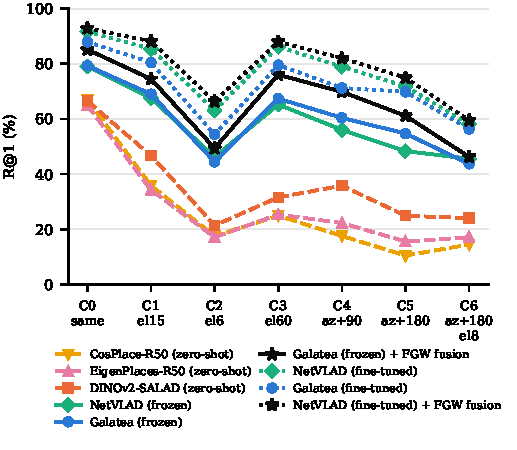
\includegraphics[width=\columnwidth]{figures/percond.pdf}
\caption{R@1 per illumination condition on the test set. Zero-shot terrestrial models (dashed)
collapse once the Sun moves. Lunar training of the aggregation head, global--local fusion and joint
backbone fine-tuning (dotted) each recover part of the loss; grazing light (C2) and reversed grazing
light (C6) remain the hardest conditions.}
\label{fig:percond}
\end{figure}
